In Fig.~\ref{fig:wg1_mjj-llLO}, we show the distributions in the invariant mass of the tagging-jet (left) and lepton-pair (right).
In both cases we show the absolute distributions in the upper plot, while the lower plot displays the ratio over {\sc VBFNLO}.
For both observables we find a relatively good agreement among the various tools, which confirms the fact that contributions from $s-$channel diagrams as well as from non-resonant configurations are strongly suppressed in the fiducial region.
We have checked that the same level of agreement holds for many other differential distributions.


 \begin{figure}[h!]
   \centering
   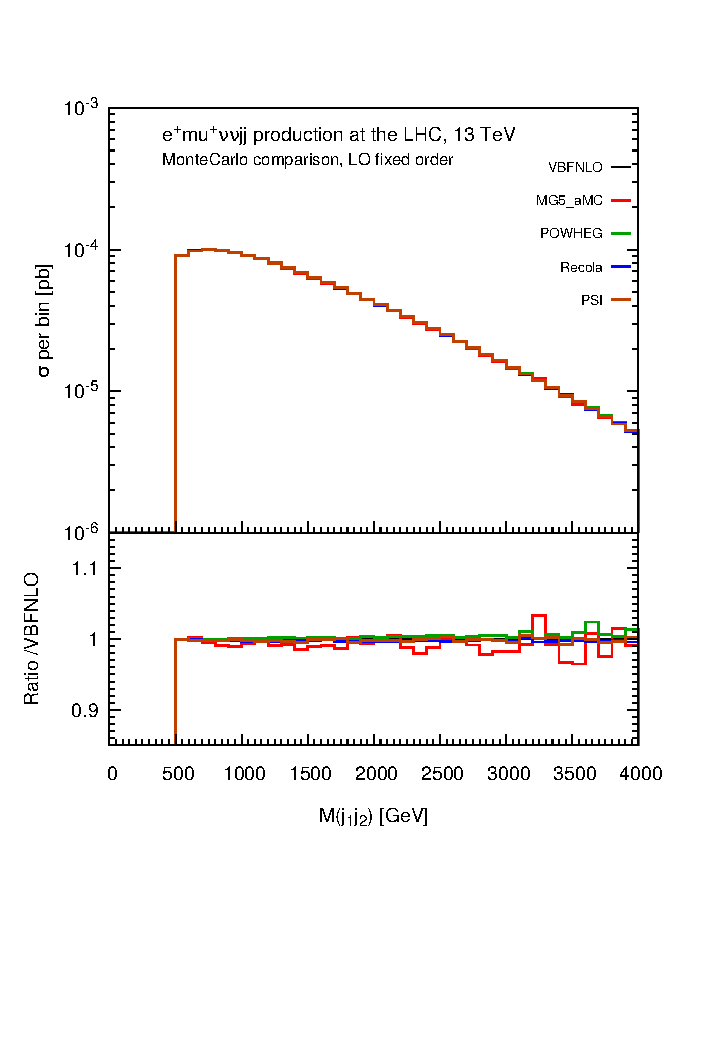
\includegraphics[width=0.4\textwidth,angle=0,clip=true,trim={0.4cm 2.5cm 0.cm 1.cm}]{figures/mjj_LO.pdf}
   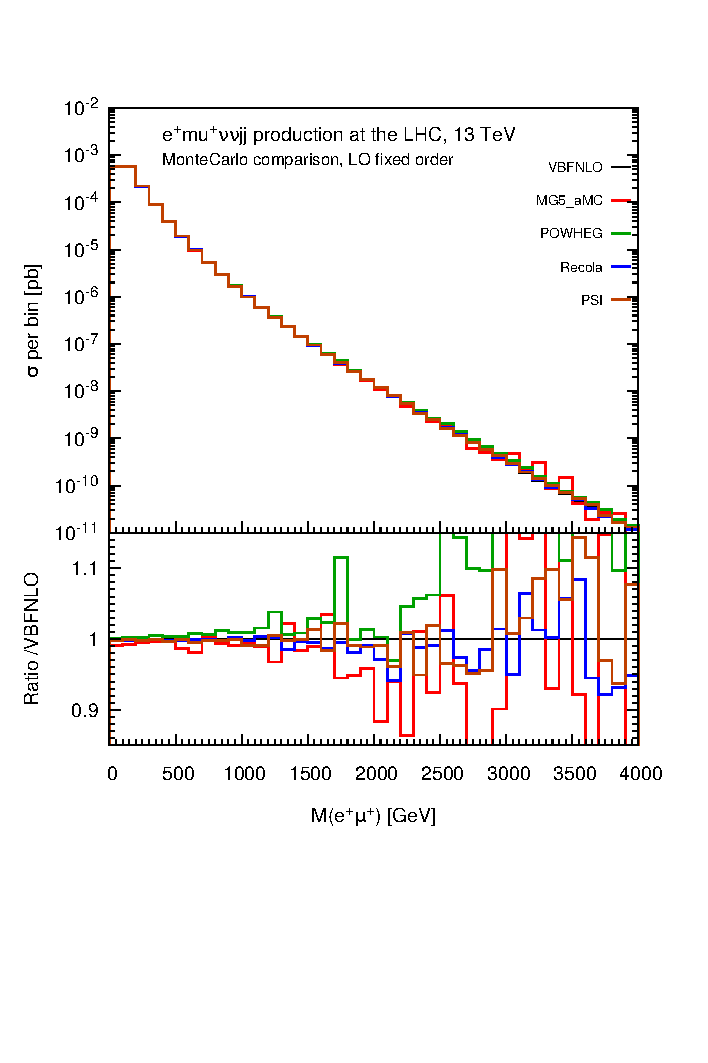
\includegraphics[width=0.4\textwidth,angle=0,clip=true,trim={0.4cm 2.5cm 0.cm 1.cm}]{figures/mll_LO.pdf}
\caption{\label{fig:wg1_mjj-llLO} Invariant-mass of the two tagging jets (left) and of the two leptons (right), at LO accuracy, 
computed with the different codes used in this comparison. The inset shows the ratio over {\sc VBFNLO}.
}
\end{figure}
